\documentclass[../main.tex]{subfiles}
\begin{document}

\chapter{Lecture 15 - 04-05-2020}
 
 \section{Regret analysis of OGD}
 We introduce the \bred{Regret}.
 \\
 $$
 \frac{1}{m} \ \sum_{t=1}^{T} \ell_t(w_t) - \frac{1}{T} \ \sum_{t=1}^{T} \ell_t(u^*_t) 
 $$
$$
(x_1,y_1) ...(x_t,y_t) \qquad \ell_t(w) = \left( w^T \, x_t - y_t\right)^2
$$
we build a loss function for example with the square loss.
\\
The important thing is that $\ell_1 , \ell_2, ...$ is a sequence of \textbf{convex losses}.
\\\\
In general we define the regret in this way:
$$
 R_T(u) \ = \ \frac{1}{m} \ \sum_{t=1}^{T} \ell_t(w_t) - \frac{1}{T} \ \sum_{t=1}^{T} \ell_t(u_t) 
$$\\
The Gradiant descent is one of the simplest algorithm for minimising a convex function. We recall the iteration did by the algorithm:
$$
w_{t+1} \leftarrow w_t - \eta_t \nabla f(w_t) \qquad \eta_t > 0 \textbf{  learning rate} \quad \textit{f convex} 
$$
$$
f: \barra{R}^d \rightarrow \barra{R} \textit{ that's why use the gradiand instead of the derivative}
$$
Learning rate can depend on time and we approach the region of the function f where the region is 0. We keep on moving in the X axes in the direction where the function is decreasing.
\newpage
\subsection{Projected OGD}

2 parameters: $\eta > 0$ and $U > 0$
\\
Initialisation: $ w_1 = (0,...,0)$
\\
For $t = 1,2,...$

1) \blue{Gradiant step}: 
$$w'_{t+1} = w_t - \frac{\eta}{\sqrt[]{t}} \ \nabla \ell_t(w_t) \qquad (x_t, y_t) \rightsquigarrow \ell_t
$$
\begin{figure}[h]
    \centering
    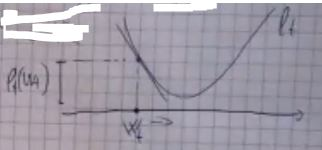
\includegraphics[width=0.3\linewidth]{../img/lez15-img1.JPG}
    \caption{}
    %\label{fig:}
\end{figure}\\

2) \blue{Projection step}: $$
w_{t+1} = arg \min_{w: \| w \| \leq U} \| w- w'_{t+1} \| $$ \textbf{Projection of $w'_{t+1}$ onto the ball of radius $U$}.
\begin{figure}[h]
    \centering
    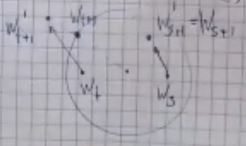
\includegraphics[width=0.3\linewidth]{../img/lez15-img2.JPG}
    \caption{}
    %\label{fig:}
\end{figure}\\
Now we define the Regret:
$$
U^*_T = arg \min_{U \in \barra{R}^d \ \|U \| \leq U} \frac{1}{T} \ \sum_{t=1}^{T} \ell_t(U)
$$
We are interested in bounding the regret $R_T\left(U^*_T\right) $
\\\\
I will Fix $\ell_1, ... \ell_t$ \qquad let $U= U^{\divideontimes}_T$ for $U$.
\\
Taylor's theorem for multivariate functions\\
Let's look a univariate first \quad $f: \barra{R} \rightarrow \barra{R}$ \textit{( has to be twice differentiable) }\qquad $w, u \in \barra{R}$
$$
f(u) = f(w) + f'(w) \, (u-w) + \frac{1}{2} \, f^"(x) \, (u-w)^2
$$
\\\\
For the multivariate case:
\\
$f: \barra{R}^d \rightarrow \barra{R} \quad$ twice differentiable \ $ \forall u, w \in \barra{R}^d$
$$
f(u) = f(w) + \nabla f(w)^T \, (u-w) + \frac{1}{2} \left(u-w\right)^T \nabla^2 f(\xi) \, (u-w)
$$
where $\xi$ is some point on the segment goining $u$ and $w$.
We have the Hessian matrix of $f$:
$$
\nabla^2 f(x)_{ij} \ = \ \frac{\partial^2 f(x)}{\partial x_i \, \partial x_j} \vert x=x_i
$$
If $f$ is convex then, $\nabla^2 f$ is positive and semidefinite.\\
$
\forall x \in \barra{R}^d \quad \forall z \in \barra{R}^d \qquad z^T \, \nabla^2 f(x) \, z \geq 0
$
\begin{figure}[h]
    \centering
    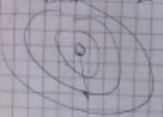
\includegraphics[width=0.3\linewidth]{../img/lez15-img3.JPG}
    \caption{}
    %\label{fig:}
\end{figure}\\

min. 38:38
\end{document}